%TODO:
%why you do the modelling and why synthesis of constraints and why properties? 

In this section, we first describe the \textit{Message authenticated CAN} (MaCAN) protocol \cite{KO15}, which is a broadcast authentication protocol specifically designed for CAN. Then, we briefly describe the \textit{Parametric Timed Automata} framework that we use to model such a protocol.    

\subsection{MaCAN protocol}
%It is backward compatible with deployed technology. 
The MaCAN protocol was designed to increase the security of the standard CAN bus. It enables incorporation of authentication message in CAN frames, which can be verified by either a single or a group of receiving nodes (ECUs). The protocol uses a new partitioning scheme that allows addition of CAN-ID (sender's ECU ID), two flag bits (for distinguishing different message types), and destination node's ID to the traditional CAN frame. The CAN-ID contains six bit source ID (src\_id) that enables the receiving node to identify the sender's node. The flag bits are mapped to the first two most significant bits of the first byte of the data field and rest six bits are used for storing destination node's ID (dst\_id). The remaining seven bytes of the crypt frame data field store the message to be transmitted. The protocol uses different format of messages, details of which can be found in \cite{KO15}.     
\vspace*{-0.15in}
\begin{figure}[h]
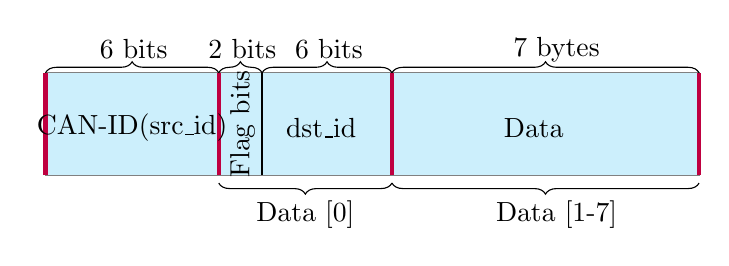
\begin{tikzpicture}
\draw[draw=black!50, fill=cyan!20] (-1, 0.2) rectangle (7.3, 1.5);
\draw [purple,ultra thick] (-1, 0.2) -- (-1,1.5) ;
\draw [purple,ultra thick] (1.2, 0.2) -- (1.2,1.5) ;
\node at (0.1,0.8) {CAN-ID(src\_id)};
\node[rotate=90] at (1.5,0.85) {Flag bits};
\draw [black,thick] (1.75, 0.2) -- (1.75,1.5) ;
\node at (2.5,0.8) {dst\_id};
\draw [purple,ultra thick] (3.4, 0.2) -- (3.4,1.5) ;
\node at (5.2,0.8) {Data};
\draw [purple,ultra thick] (7.3, 0.2) -- (7.3,1.5) ;
\draw [rotate=0,decorate,decoration={brace,amplitude=4pt}]
(-1,1.5) -- (1.2,1.5);
\node at (0.12,1.8) {6 bits};
\draw [rotate=0,decorate,decoration={brace,amplitude=4pt}]
(1.2,1.5) -- (1.75,1.5);
\node at (1.5,1.8) {2 bits};
\draw [rotate=0,decorate,decoration={brace,amplitude=4pt}]
(1.75,1.5) -- (3.4,1.5);
\node at (2.6,1.8) {6 bits};
\draw [rotate=0,decorate,decoration={brace,amplitude=4pt}]
(3.4,1.5) -- (7.3,1.5);
\node at (5.49,1.8) {7 bytes};
\draw [decorate,decoration={brace,mirror,amplitude=4pt}]
(3.4,0.1) -- (7.3,0.1);
\node at (5.49,-0.3) {Data [1-7]};%  %% Grid lines 
\draw [decorate,decoration={brace,mirror,,amplitude=4pt}]
(1.2,0.1) -- (3.4,0.1);
\node at (2.3,-0.3) {Data [0]};
%     \draw[help lines] (-1, -1) grid (7.3, 1);
%   \foreach \i in {-1,...,7} {
%         \node[anchor=north] at(\i, -1) {\footnotesize \i};
%     }
%     \foreach \i in {-1, ...,1} {
%         \node[anchor=east] at (-1, \i) {\footnotesize \i};
%     }
\end{tikzpicture}
\vspace*{-0.1in}
\caption{Crypt Frame} \label{fig:cframe}
\end{figure}
\vspace*{-0.15in}

The MaCAN protocol requires a \textit{key server} (KS) for distributing key among the nodes and a \textit{time server} (TS) to synchronize internal counter of nodes with the global time. The KS maintains the session keys and stores the symmetric long-term keys (LTK) of all the nodes (ECUs) of the vehicle network. The TS periodically provide precise time to all the nodes and respond to authenticated time request. With this setup, the protocol performs three procedures: (i) session key establishment, (ii) signal authentication, and (iii) time synchronization, for secure message transmission in CAN network.               

\vspace*{0.1in}
\noindent \underline{\textit{Session Key Establishment}}

\vspace*{0.05in}
Prior to the exchange of authenticated messages among ECUs (nodes), the MaCAN protocol requires the sender ($ECU_i$) and the receiver ($ECU_j$) nodes to obtain a session key by communicating with the \textit{key server}. Figure. \ref{fig:skest} illustrates the key establishment procedure. To send the session keys to the nodes, the \textit{key server} uses the stored LTK of ($ECU_i$) and ($ECU_j$).

The procedure starts with $ECU_i$ sending a challenge $C_i$ and ID $id_j$ of the node it wants to communicate with to the \textit{KS} (\ref{ske1}). The \textit{KS} respond by sending \textbf{SK} message that contain the fresh session key $SK_{ij}$, the challenge $C_i$, and IDs of $ECU_i$ ($id_i$) and $ECU_j$ ($id_j$), encrypted with the LTK $K_{i, LTK}$ of $ECU_i$ (\ref{ske2}). Subsequently, \textit{KS} sends
a request for challenge (\textbf{RC}) to $ECU_j$, notifying it of the session key that has been generated (\ref{ske3}). After $ECU_i$ decrypts the session key $SK_{ij}$ and verify the challenge value, it sends an acknowledgement message \textbf{ACK} to $ECU_j$. The \textbf{ACK} message consist of a 24-bit group field $gf$ that indicates the nodes the sender ($ECU_i$) is aware of being authenticated and a signed (with $SK_{ij}$) cipher based message authentication code (\textit{cmac}) that includes the current timestamp $T$, the group field, and ID of $ECU_j$ (\ref{ske4}). Subsequently, $ECU_j$ follows an analogous procedure to obtain the session key from the key server and notify $ECU_i$ (\ref{ske5}, \ref{ske6}, \ref{ske7}). When $ECU_i$ verifies the authenticity of the \textbf{ACK} message received from $ECU_j$ and does not find its ID in the group field, it sends another \textbf{ACK} to $ECU_j$ with both $id_i$ and $id_j$ bits in the group field set (\ref{ske8}).     
%informing it of the received session key
\vspace*{-0.15in}
\begin{figure}[h]
\begin{align}
 ECU_i \rightarrow KS &: \mathbf{CH}, C_i, id_j \label{ske1}\\ 
 KS \rightarrow ECU_i &: \mathbf{SK}, \{C_i, id_j, id_i, SK_{ij}\}_{K_{i,LTK}} \label{ske2}\\
 KS \rightarrow ECU_j &: \mathbf{RC}, id_i \label{ske3}\\ 
 ECU_i \rightarrow ECU_j &: \mathbf{ACK}, gf(id_i),\{cmac(T, id_j, gf(id_i))\}_{SK_{ij}} \label{ske4}\\
 ECU_j \rightarrow KS &: \mathbf{CH}, C_j, id_i \label{ske5}\\
 KS \rightarrow ECU_j &: \mathbf{SK}, \{C_j, id_j, id_i, SK_{ij}\}_{K_{j,LTK}} \label{ske6}\\
ECU_j \rightarrow ECU_i &: \mathbf{ACK}, gf(id_j), \{cmac(T, id_i, gf(id_j))\}_{SK_{ij}} \label{ske7}\\
ECU_i \rightarrow ECU_j &: \mathbf{ACK}, gf(id_i|id_j), \{cmac(T, id_j, gf(id_i|id_j))\}_{SK_{ij}} \label{ske8}
\end{align}
\vspace*{-0.2in}
\caption{MaCAN session key establishment procedure} \label{fig:skest}
\end{figure}

\vspace*{-0.1in}
The MaCAN protocol supports authentication of groups with more than two ECUs. The groups are formed by members with same trust level (e.g. ECUs made by the same manufacturer can form a group) and they share the same session key for message exchange.    

\vspace*{0.1in}
\noindent \underline{\textit{Signal Authentication}}

\vspace*{0.05in}
After establishing the session keys, the ECUs communicate with each other by periodically exchanging messages with signal values (e.g. sensor data of tire pressure is a signal). To receive a signal $sig\#$, the receiving node $ECU_i$ should first send an authenticated signal request $\mathbf{SIG\_AUTH\_REQ}$ message to node $ECU_j$ (\ref{sa1}). The request message is a signed $cmac$ that includes the signal number $sig\#$ that needs to be authenticated, \textit{presc} that specifies the signing behavior ($presc =0$: request the next message to be authenticated, $presc =1$: request each following message to be authenticated), the current time stamp $T$, and the sender and receiver node's IDs. After verifying the $cmac$, $ECU_j$ sends the $\mathbf{AUTH\_SIG}$ message that contains the signed signal value $Signal$ to $ECU_i$ (\ref{sa2}).                  

\vspace*{-0.15in}
\begin{figure}[ht]
\begin{align}
 ECU_i \rightarrow ECU_j &: \mathbf{SIG\_AUTH\_REQ}, sig\#, presc, \nonumber \\ 
                         &\{cmac(T, id_i, id_j, sig\#, presc)\}_{SK_{ij}} \label{sa1}\\
 ECU_j \rightarrow ECU_i &: \mathbf{AUTH\_SIG}, sig\#, Signal, \nonumber \label{sa2}\\ 
                         &\{cmac(T, id_i, id_j, sig\#, Signal)\}_{SK_{ij}} 
\end{align}
\vspace*{-0.2in}
\caption{MaCAN signal authentication procedure} \label{fig:sauth}
\end{figure}

\vspace*{-0.1in}
\noindent \underline{\textit{Time Synchronization}} 

\vspace*{0.05in}
The ECUs of the MaCAN protocol uses time $T$ as one of the inputs in the $cmac$ function. As such, each ECU has an internal clock that is synchronized to the global clock of the \textit{time server (TS)}. The global time is broadcasted periodically in an unauthenticated form by the $TS$. Every ECU receives the time signal and compare it against its internal clock value. If there is a large mismatch between the time values, then the ECU request $TS$ for an authentic time value by sending a challenge message $\mathbf{CH}$ with $fwd\_id$ set to $0$ and the challenge $C_i$ (\ref{tau1}). Subsequently, the $TS$ responds with the authenticated time $\mathbf{AT}$ message, which is signed with the ECU's session key $SK_{ij}$ and contains the last broadcasted timestamp value $T$ and the challenge $C_i$ (\ref{tau2}).                  

\vspace*{-0.15in}
\begin{figure}[ht]
\begin{align}
 ECU_i \rightarrow TS &: \mathbf{CH}, C_i, fwd\_id = 0 \label{tau1} \\ 
 TS \rightarrow ECU_i &: \mathbf{AT}, T, \{cmac(T, C_i)\}_{SK_{i,TS}} \label{tau2}
\end{align}
\vspace*{-0.2in}
\caption{MaCAN time synchronization procedure} \label{fig:tauth}
\end{figure}

\vspace*{-0.1in}
As each communication signal (or message) of the network uses the current time value, attack such as replay can be detected and ECUs can be prevented from being affected by corrupted messages. 

\subsection{Modeling of Security Protocol}

% To ascertain the MaCAN protocol abide by the timing properties of the vehicle network, we first model the protocol using the formalism of \textit{Parametric Timed Automata}, which is an extension of the class of Timed Automata. Then, we find the bounds on the parameters   
Next, we use the formalism of \textit{Parametric Timed Automata} (PTA), which is an extension of the class of Timed Automata (TA) to model the protocol ~\cite{BBHBC14}. Unlike TA that uses \textit{constants} in the clock constraints, the PTA allow use of \textit{parameters} i.e. unknown constants within these constraints.

\begin{definition}
A \textit{PTA} is a tuple of the form $\mathcal{M} = (\Sigma, L, l_0, X, P, I, E, K)$, where $i) \; \Sigma$ is a finite set of actions, $ii) \; L$ is a finite set of locations, $iii) \;l_0 \in L$ is the initial location, $iv) \; X$ is a finite set of non-negative real valued $\mathbb{R}^+$ clocks, $v)\; P$ is a finite set of $\mathbb{R}^+$ parameters, $vi)\; I$ is the invariant that assign a guard  $g(X)$ - constraint over $(X, P)$ of the form $x \sim p$, where $\sim \, \in \{ <, \leq, \geq , > \}$ - to every $l \in L$, $vii) \;E$ is a set of edges $e = (l, g, a, R, l')$ where $l, l' \in L$ are the source and destination locations, $a \in \Sigma$, $g$ is a guard, and $R \subseteq X$ is a set of clocks to be reset, and $viii) \;K$ is a constraint over $P$.    
\end{definition}

\raj{Implement the model in IMITATOR}
% relate the PTA to the security protocol. 
% assumptions while modeling the protocol such as use of counter for timeouts between transition and action to take when timeout.
% assumption : we have the platform independent model 